\chapter{Results}
\label{ch:results}

This chapter presents the results of the project, structured according to the two main research questions: (1) how design theories can improve dashboard usability, and (2) how iterative development enhances functionality and user experience. The findings comprise qualitative feedback, quantitative metrics, design outcomes, and requirement fulfilment. 

\section{Usability and Design Improvements (RQ1)}
This section addresses the first research question by presenting both qualitative and quantitative findings related to the dashboard’s usability, as well as how user feedback and design principles influenced the final interface.


\subsection{Final Application Design Outcomes}
\label{subsec:final_app_design_results}

Design refinements, implemented in response to user feedback, were grounded in the design theories discussed in Chapter~\ref{ch:theory} (e.g., Nielsen’s heuristics, Norman’s interaction design principles, and Few’s dashboard guidelines). The resulting interface aimed to balance information density with clarity, using dynamic ordering of dashboard cards, status indicators, and colour-coding to improve usability.

\subsubsection{Dashboard Page Design}
The main dashboard shown below in Figure~\ref{fig:main_dashboard}) was guided by Few’s simplicity principle and Nielsen’s aesthetic and minimalist heuristic. Information is prioritized through dynamic component ordering based on the status of the website, clear iconography, and colour-based status indicators. Gestalt principles, including proximity, enclosure, and similarity, enhanced visibility and structure, directly contributing to improved comprehension.


\begin{figure}[H]
    \centering
    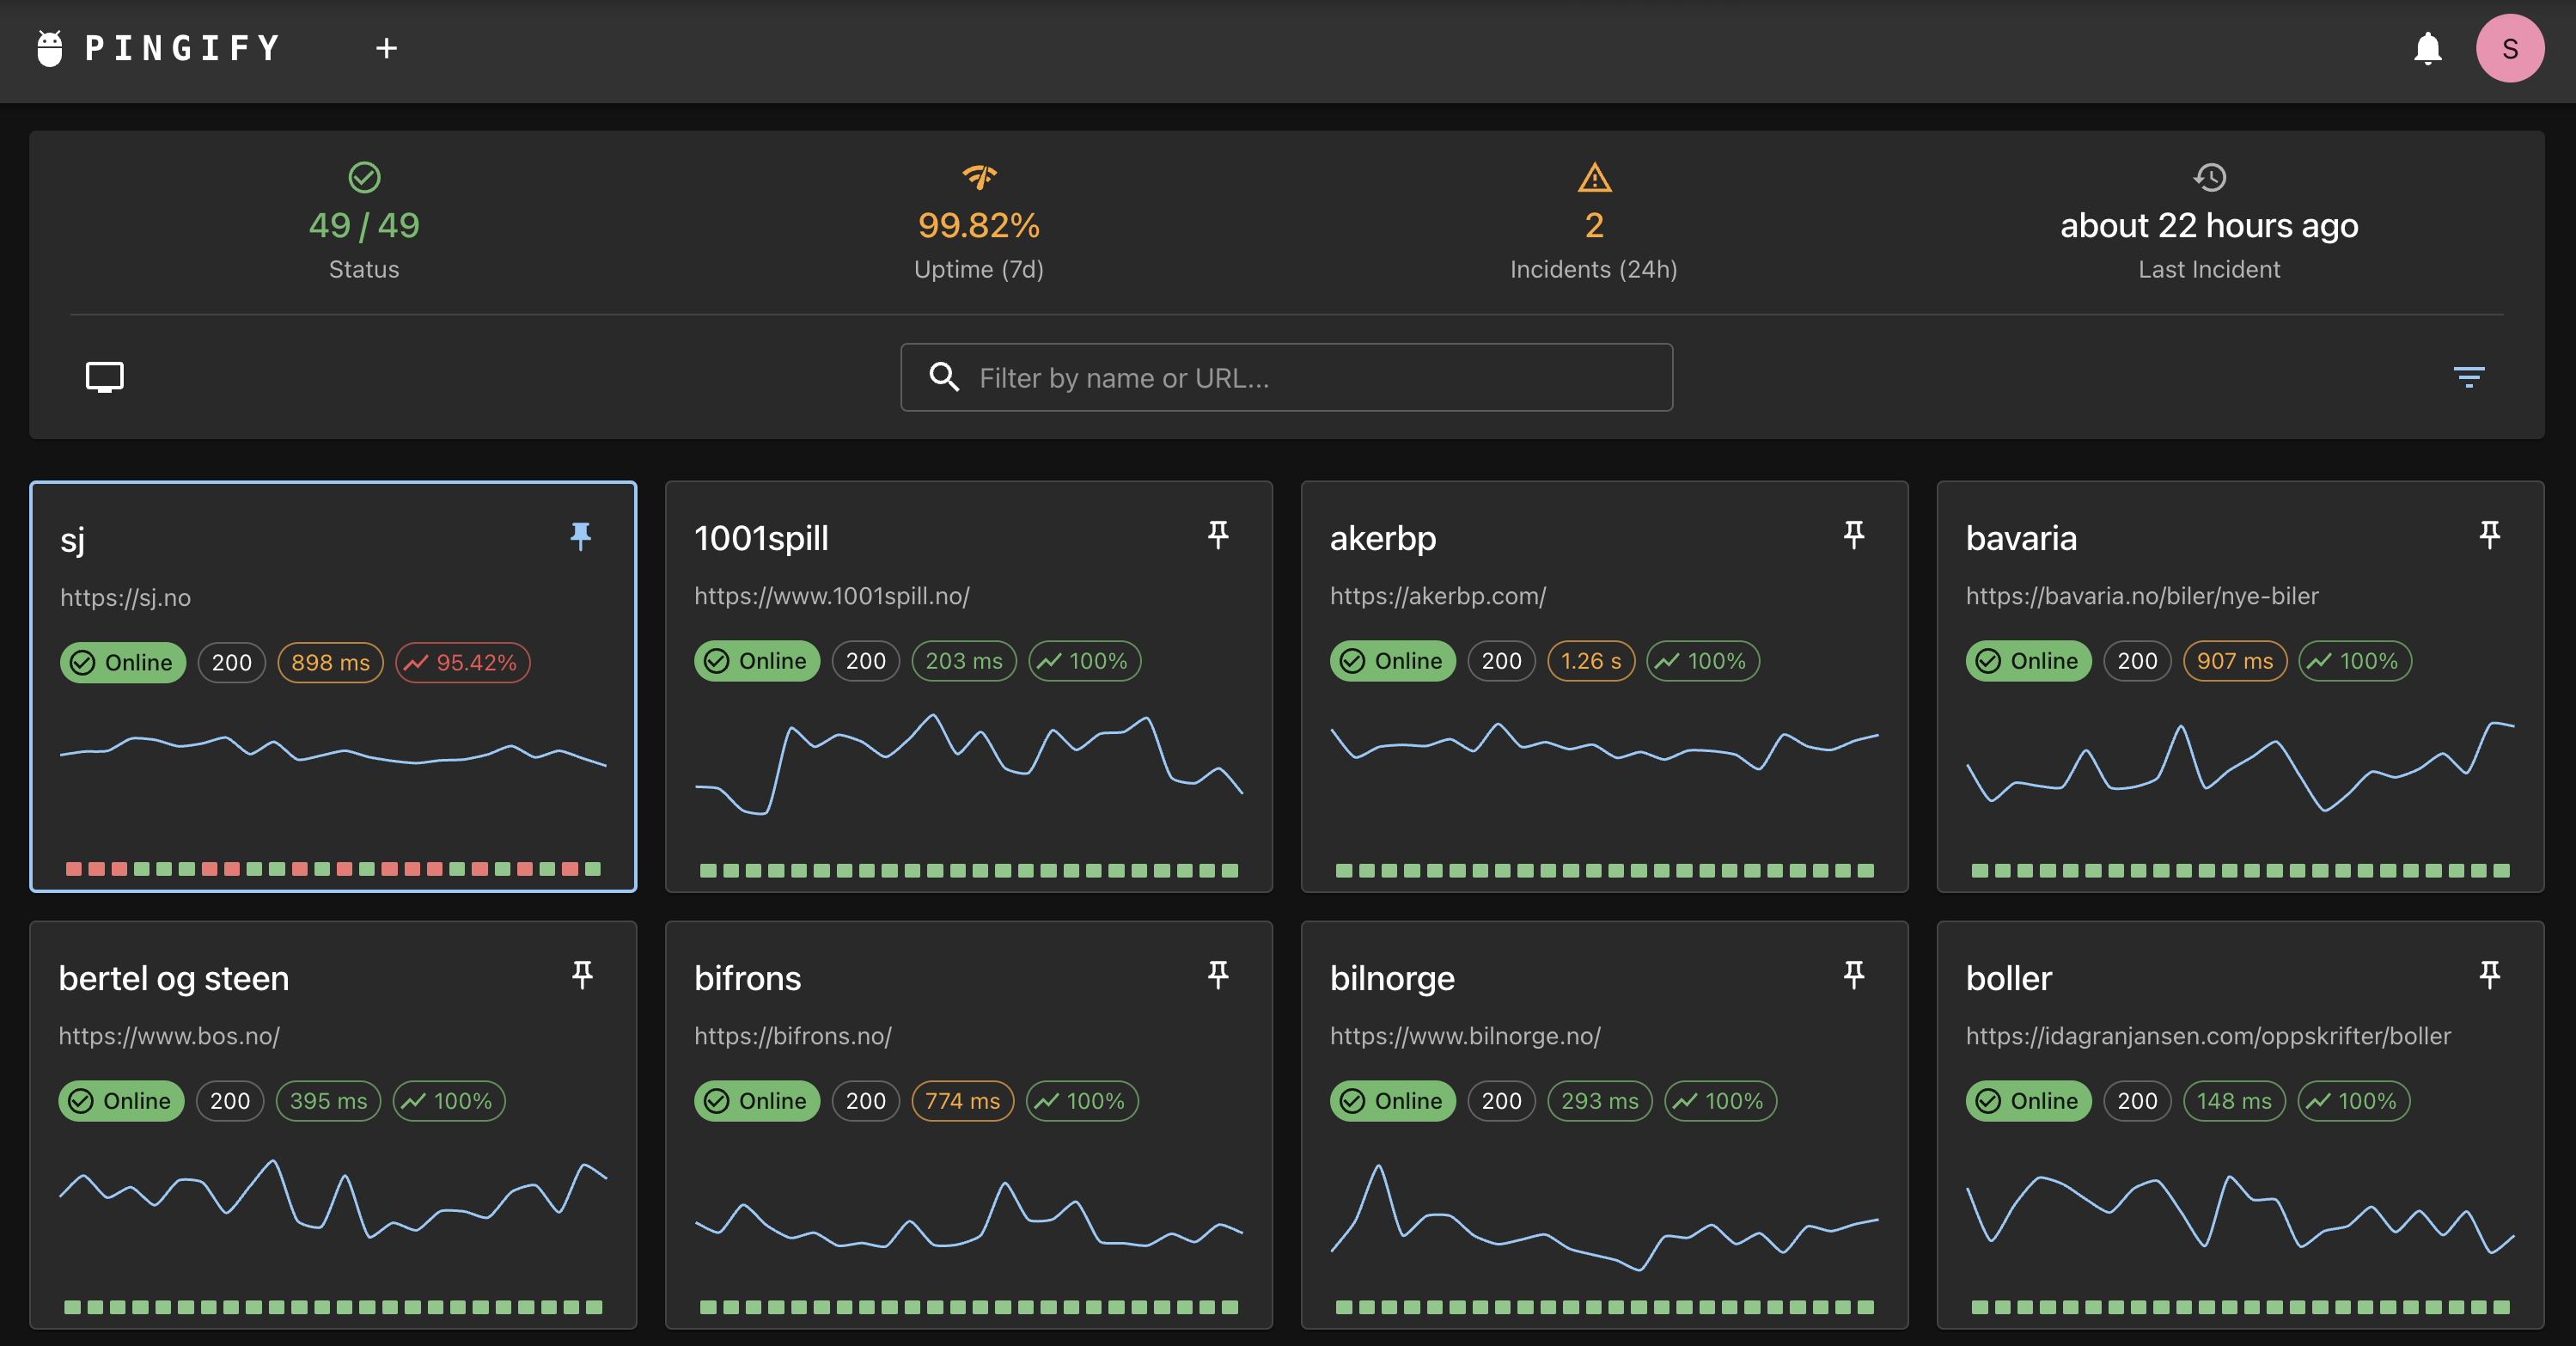
\includegraphics[width=1\linewidth]{figures/main_dashboard.png}
    \caption{Main Dashboard with Pinned Website}
    \label{fig:main_dashboard}
\end{figure}

\subsubsection{Website Card Design}
The Website Card (Figure~\ref{fig:websitecard_comparison}) displays a the status of a website using real-time indicators. Design changes addressed feedback that cards previously lacked detail (Table~\ref{tab:prototype-issues}). Each card now includes more data points and clear, consistent visual styling to reduce cognitive load. This aligns with Norman’s emphasis on usability and Nielsen’s “Consistency and Standards”~\autocite{Nielsen1994}.

\begin{figure}[H]
    \centering
    \includegraphics[width=1\linewidth]{figures/MVP-dashboard/MVP-cards.png}
    \caption{Two Website Cards: One offline and one online}
    \label{fig:websitecard_comparison}
\end{figure}

\subsubsection{Website Details Page Design}
The Website Details view supports deeper investigation of issues. It includes performance graphs, status banners, and a timeline of incidents. Visual updates address participant requests for contextual data (Table~\ref{tab:mvp-issues}) and apply Norman’s principles of visibility and feedback. As seen in the Figure~\ref{fig:website_details_results} below, the user can select different time frames for the charts (1h, 24h, 7d, 30d, 1y), review earlier incidents and latest checks. While still having control of the main status of all monitored websites in the navbar at the top.

\begin{figure}[H]
    \centering
    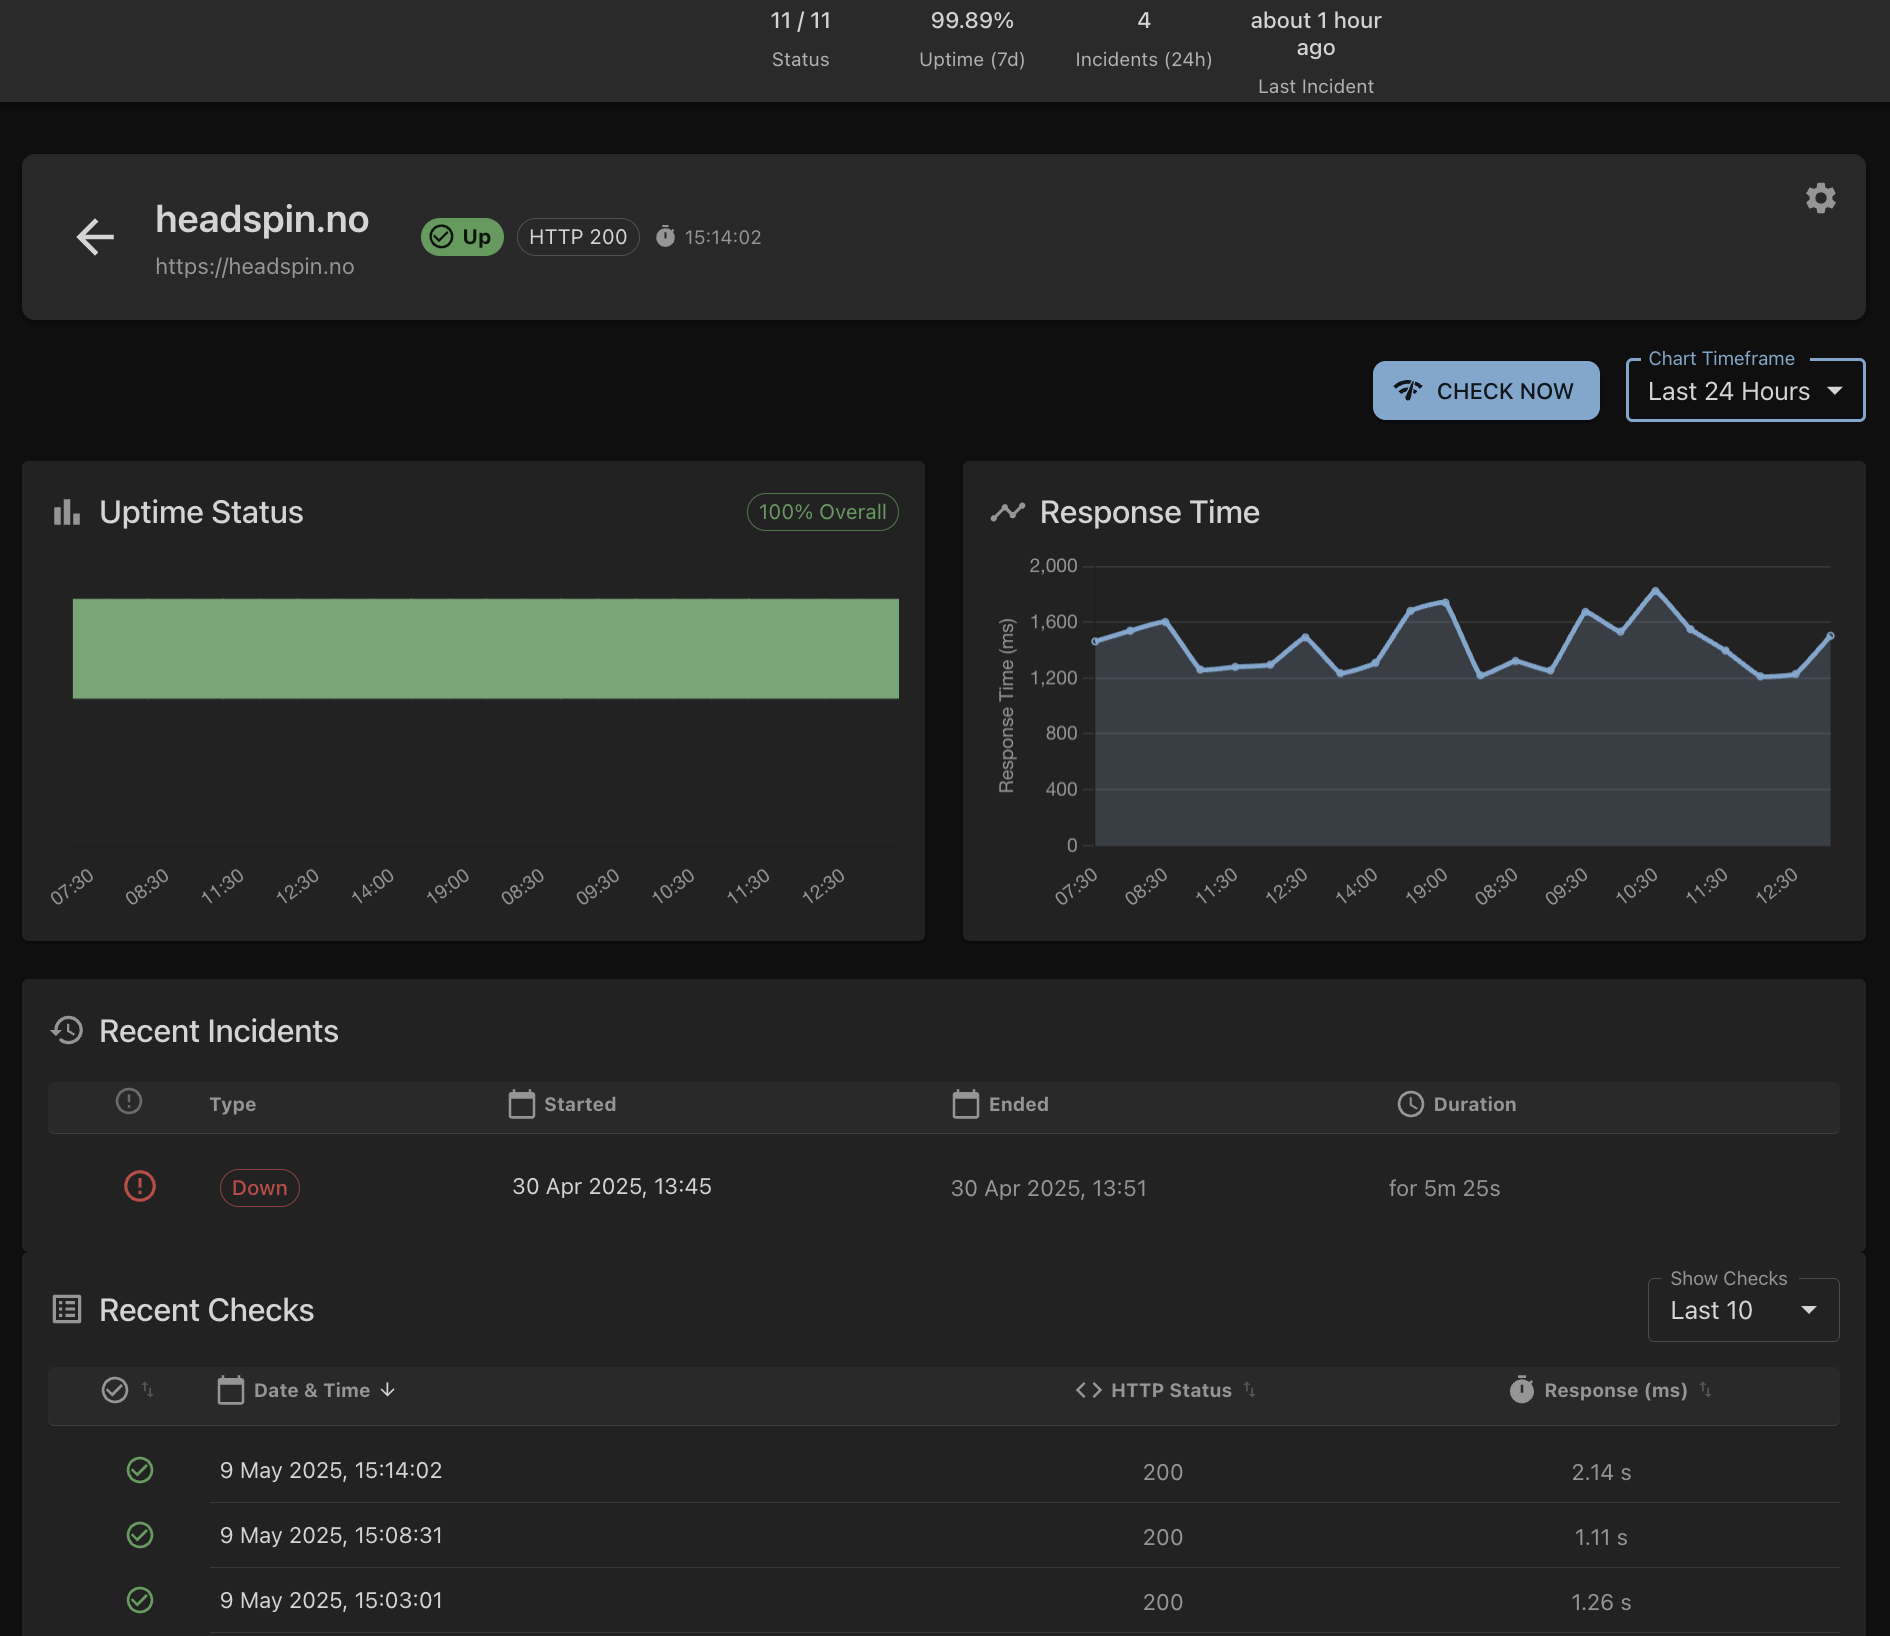
\includegraphics[width=1\linewidth]{figures/MVP-dashboard/MVP-websitedetails_full.png}
    \caption{Website Details}
    \label{fig:website_details_results}
\end{figure}

\subsubsection{Design Evolution}
The final dashboard reflects a number of significant design improvements made in response to iterative user testing. These changes not only addressed specific usability issues raised during evaluations but also implemented theoretical guidance from the design principles outlined in Chapter~\ref{ch:theory}. Below are four key examples of such refinements.

\paragraph{Navigation Bar (Navbar)}
During the first round of user testing, participants expressed confusion over the original hamburger-style side menu, which was perceived as redundant and non-intuitive. In line with Norman’s principles of affordance and visibility \parencite{sharp-2019}, this element was removed in favour of a persistent top navigation bar (Figure~\ref{fig:navbar}).

\begin{figure}[H]
    \centering
    
\includegraphics[width=1\linewidth]{figures/navbar.png}
    \caption{Navbar with changes made}
    \label{fig:navbar}
\end{figure}

The redesigned navbar now includes a home button (logo + title), a clearly labeled button for adding websites (with tooltip), an alert indicator with a numeric badge, and a profile dropdown for user settings. This reconfiguration ensures that high-frequency actions are immediately visible, adhering to Norman's principle of visibility \parencite{sharp-2019} .

To further enhance discoverability, the "Add Website" function was duplicated as a dedicated card component in the main dashboard grid (Figure~\ref{fig:addwebsitecard}). This design decision aligns with universal design principles, providing multiple access points for critical tasks.


\begin{figure}[H]
    \centering
    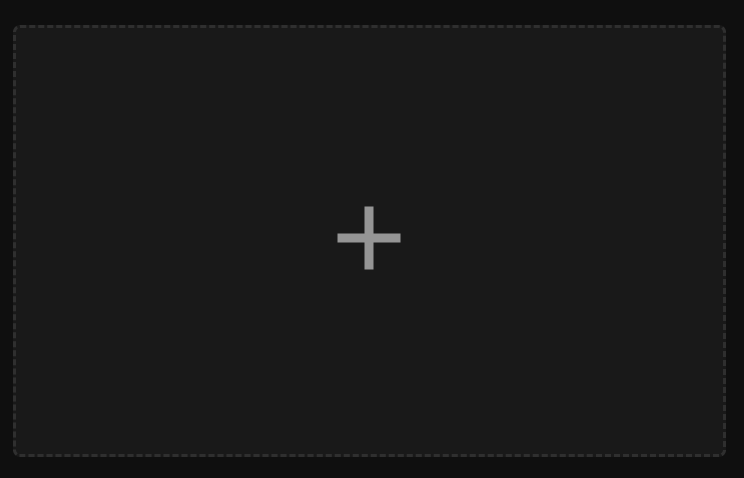
\includegraphics[width=0.5\linewidth]{figures/addwebsitecard.png}
    \caption{Add Website Card}
    \label{fig:addwebsitecard}
\end{figure}

\paragraph{Filtering and Pinning}
Feedback from user test 1 also indicated confusion around the placement of the filtering options, which were originally located in the now-removed sidebar. Following expectations based on conventional UI patterns and learned user behavior \parencite{Nielsen1994}, the filtering controls were relocated directly above the website cards on the right-hand side (Figure~\ref{fig:statusbar}).

The new placement aligns with Few’s emphasis on contextual clarity and effective use of limited screen space \parencite{FewDashboard}, ensuring that filtering tools are readily available without cluttering the interface. 

The card-sorting logic was also refined to prioritize content dynamically: pinned cards appear first, followed by down websites, then alphabetically ordered cards. This prioritization strategy uses critical value exceptions and reflects Nielsen's heuristic of visibility of system status \parencite{Nielsen1994}. 

\begin{figure}[H]
    \centering
    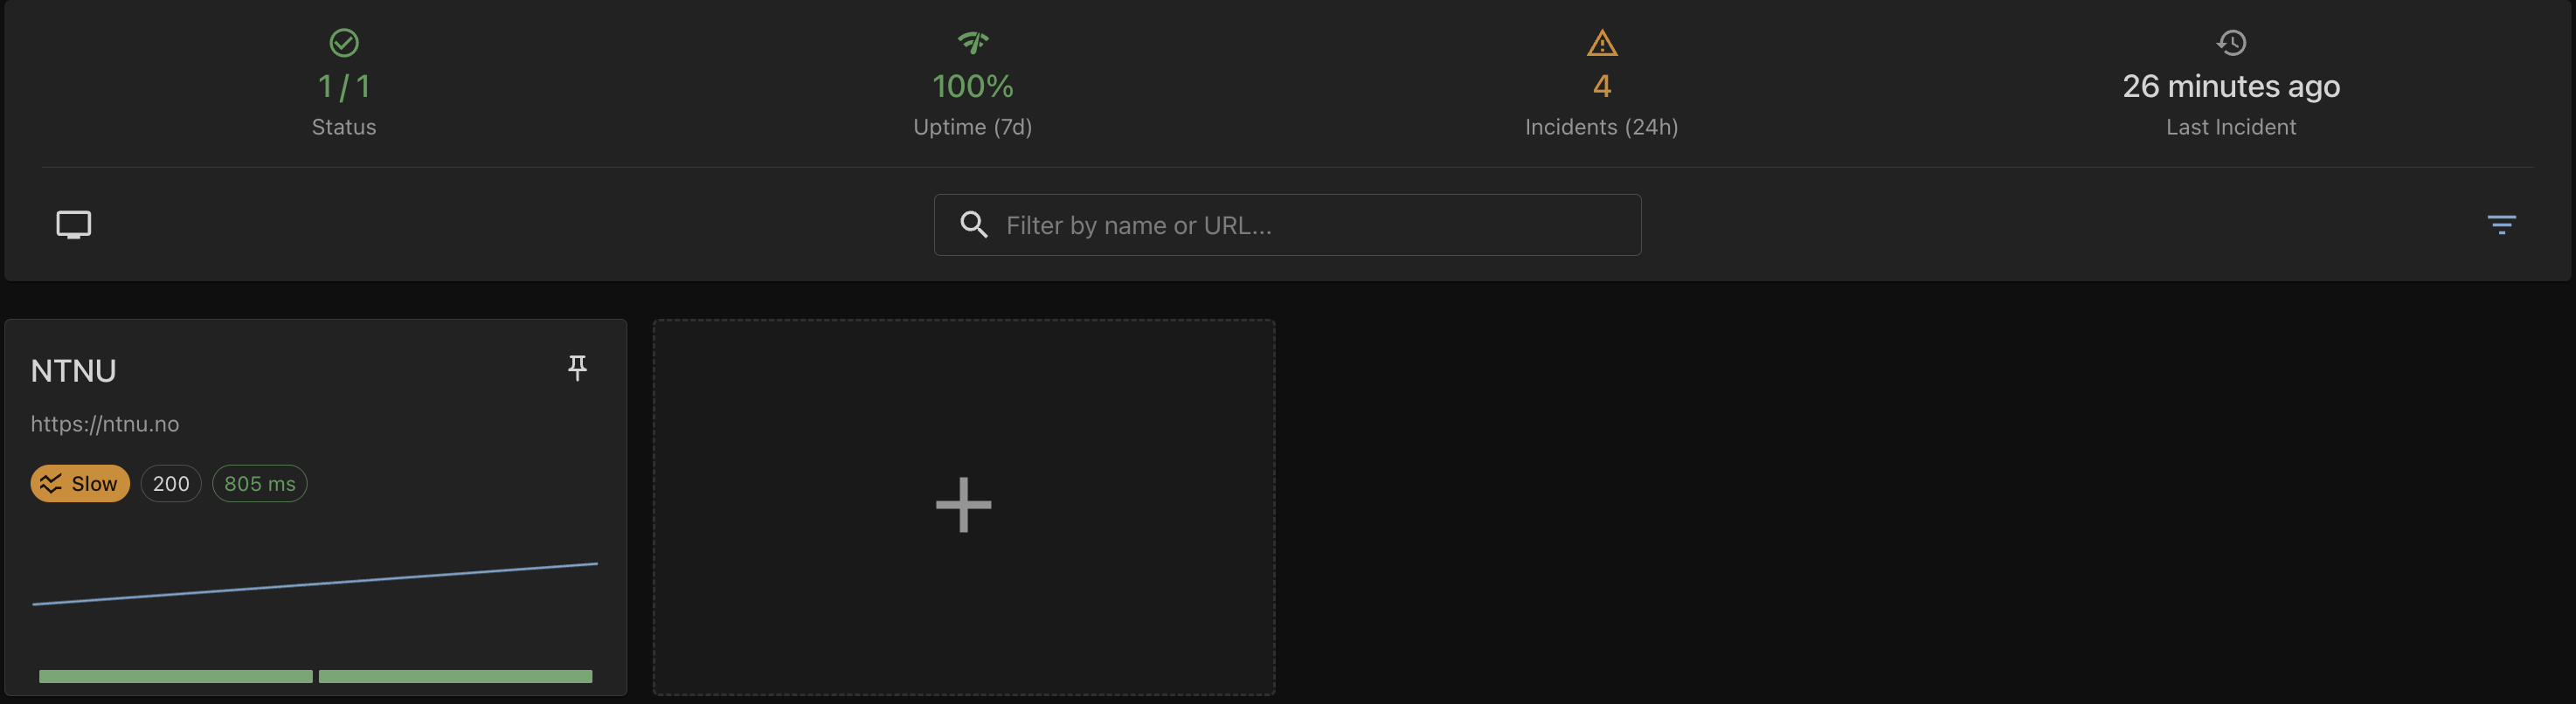
\includegraphics[width=1\linewidth]{figures/statusbar.png}
    \caption{Status Bar with TV-mode, Searchbar and Filtering}
    \label{fig:statusbar}
\end{figure}

\paragraph{TV-Mode}
TV-mode was developed in response to stakeholder and user feedback that the dashboard would often be used passively on large screens in office environments. The feature was originally labeled “Focus-mode” but was renamed and redesigned following confusion in user test 2.

As shown in Figure~\ref{fig:tv-mode}, TV-mode activates a fullscreen display, hiding both the navbar and filter bar to prioritize status cards. The icon and tooltip were redesigned after user test 2 for better affordance, following Norman’s guidelines on intuitive feedback and mapping. These changes also relate to Few’s emphasis on clarity, enabling users to monitor key metrics without distraction or interface noise.

\begin{figure}[H]
    \centering
    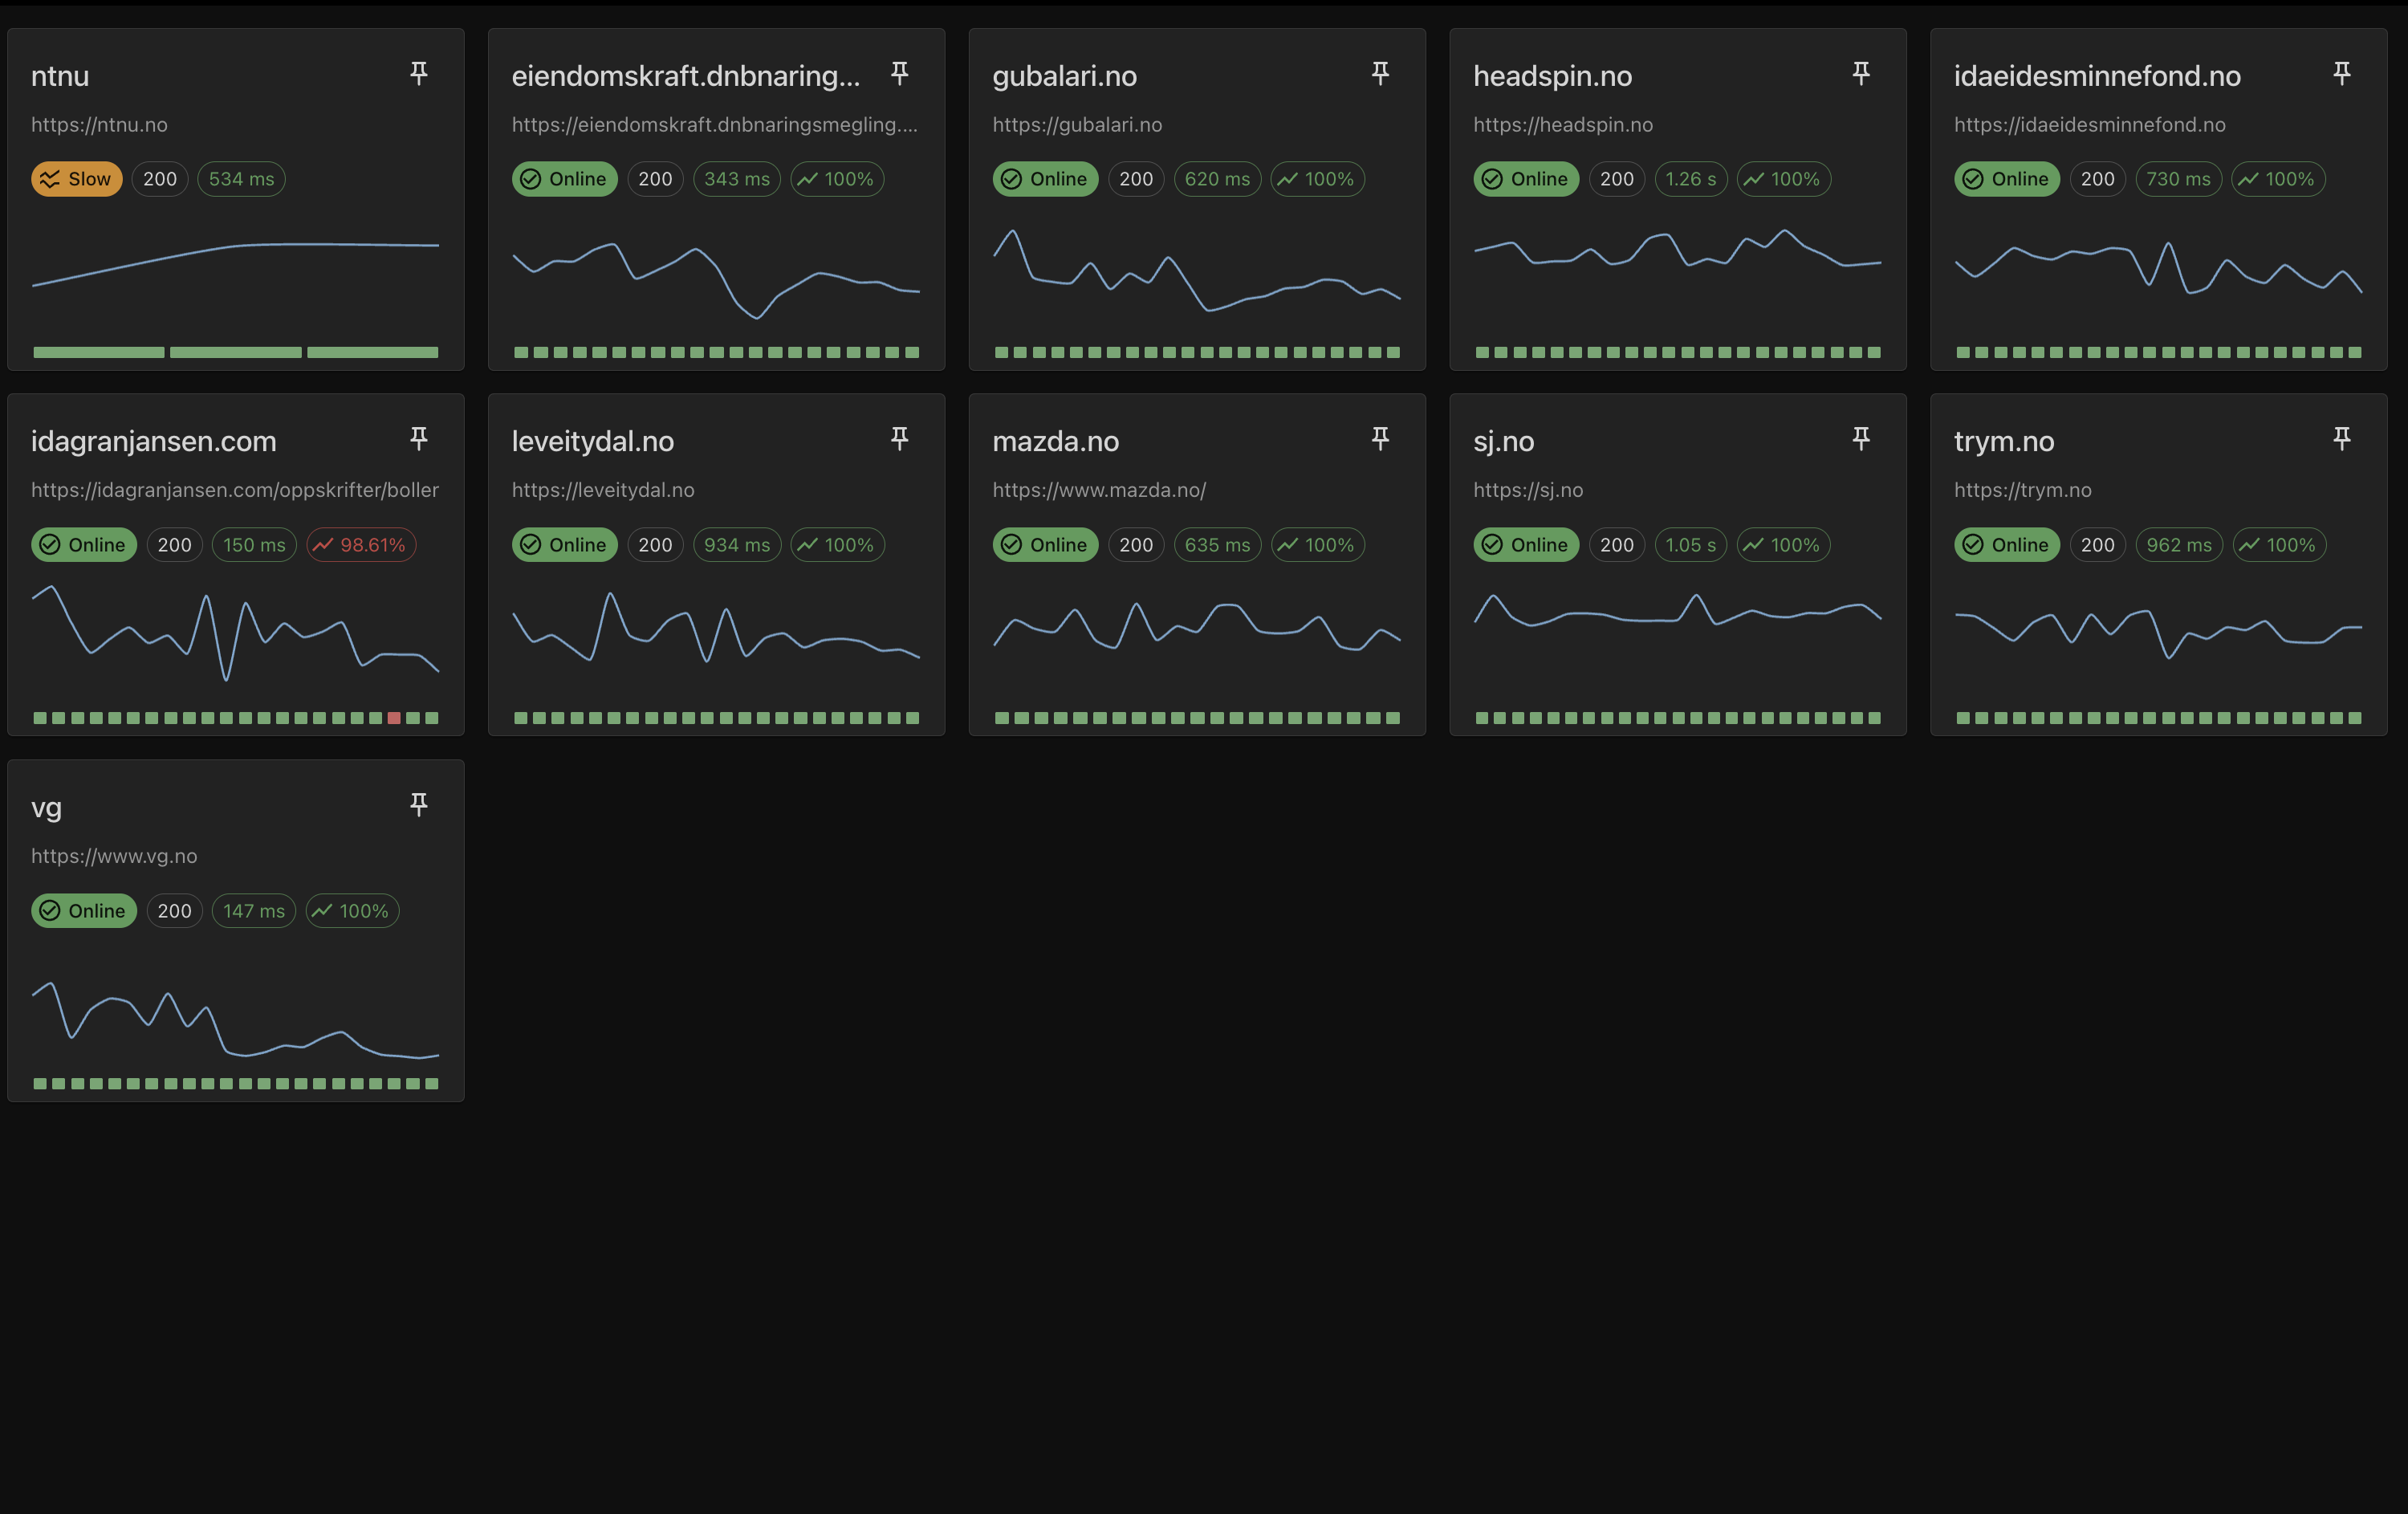
\includegraphics[width=0.75\linewidth]{figures/tv-mode.png}
    \caption{TV-Mode}
    \label{fig:tv-mode}
\end{figure}


\paragraph{Back-button in Details View}
The need for an explicit way to return from the website details page to the dashboard emerged from user test 2. Although not prioritized until later in the development process, the final application includes a dedicated back-button prominently placed in the header (Figure~\ref{fig:header_websitedetails}).

This addition applies Norman's principles of affordance and visibility and was also an important component in improving navigational consistency \parencite{sharp-2019}. It reduces cognitive load by eliminating reliance on browser controls or guessing.

\begin{figure}[H]
    \centering
    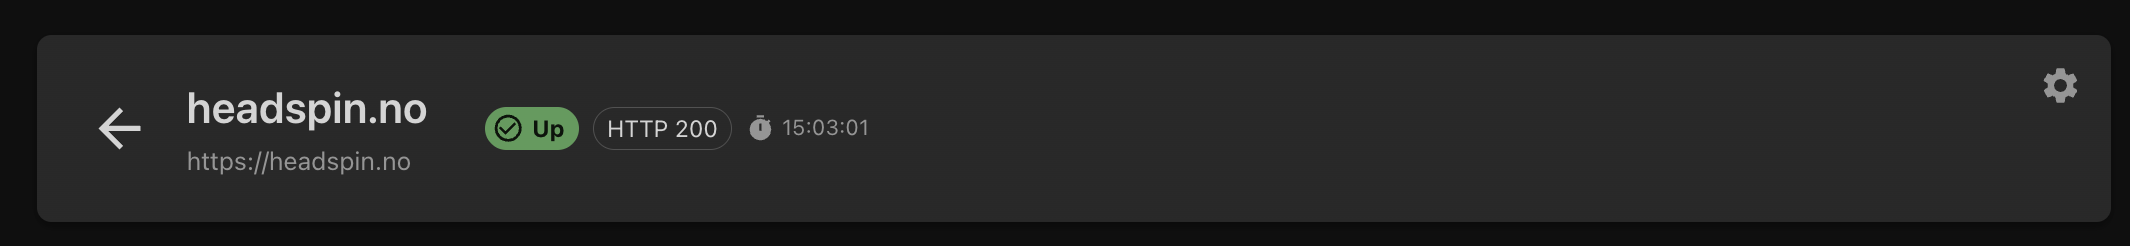
\includegraphics[width=1\linewidth]{figures/header_websiteDetails.png}
    \caption{Website Details Header with back-button, status indicators, and cogwheel for settings}
    \label{fig:header_websitedetails}
\end{figure}


\subsection{Qualitative Feedback on Usability}
User testing of both the prototype and the \acrshort{mvp} version revealed several usability insights. Participants interacted with the system and provided feedback during and after completing realistic usage scenarios.

\subsubsection{Visual Design and Colours}
Initial prototype feedback indicated issues with the colour scheme. For instance, one participant noted that \textit{“everything appeared too green and lacked visual distinction”} (Prototype User Test, P1), while another described the interface as \textit{“very green” and "somewhat cluttered”} (Prototype User Test, P2). Multiple participants agreed that \textit{“solid-green cards were visually overwhelming; smaller status indicators were preferred”} (Table~\ref{tab:prototype-issues}). These comments prompted the introduction of a revised colour scheme in the \acrshort{mvp}, aiming to improve visual hierarchy and contrast. The design update adhered to aesthetic and minimalist principles~\autocite{Nielsen1994} and addressed NF.5.

%her må vi dra inn en spesifikk ting med navigasjon of layout som endret seg pga brukerrespons I user test 1: feks filtering flyttet fra sidebar til over kortene med bruk av ikon
\subsubsection{Navigation and Layout}
During prototype testing, the sidebar navigation was deemed unnecessary by some users (\textit{“the sidebar was seen as unnecessary, and a top-mounted menu was preferred”} – P1; \textit{“a slimmer taskbar with icons was suggested”} – P3, Table~\ref{tab:prototype-issues}). In user test 1, of the prototype, the placement of the “Add Website” function in the side menu was found unintuitive (\textit{“expected as a prominent action button on the dashboard”} – P2). These findings informed subsequent layout refinements, enhancing navigational clarity.


\subsubsection{Data Readability and Information Density}
Participants of user test 1 expressed a need for more compact visualisations and denser information displays. One participant highlighted the importance of \textit{“metrics like response time in milliseconds and uptime percentages over different time ranges (day, month, year)”} (P1). Others commented that \textit{“each site card showed too little information”} (P3). In response, the final design integrated historical data features (F.3, F.8) and refined visual indicators. However, in the user test 2, the inclusion of more data led to additional feedback regarding graph interpretability (\textit{“It was unclear what the main graph represented”} – P1).

\textit{Detailed feedback from the prototype and \acrshort{mvp} stages is summarised in Tables~\ref{tab:prototype-issues} and~\ref{tab:mvp-issues}, respectively.}


\subsubsection{Prototype table}
\begin{table}[H]
\centering
\begin{tabular}{|p{8.2cm}|c|}
\hline
\textbf{Issue raised by participants} & \textbf{Reported by} \\ \hline
Each card showed too little information; more detail was requested.& P1, P2, P3 \\ \hline
Solid‑green cards were visually overwhelming; smaller status indicators were preferred. & P1, P2, P3 \\ \hline
A list view was preferred over cards to reduce visual clutter. & P2 \\ \hline
Need for historical status data (day/week/month/year) to see trends. & P1, P2 \\ \hline
Cards should include icons and key contact info (adviser, developer, favicon). & P2 \\ \hline
Option to pin or feature important sites at the top of the dashboard. & P3 \\ \hline
Sidebar (hamburger menu) was viewed as unnecessary; top navigation or slimmer icon bar was preferred. & P1, P3 \\ \hline
Dashboard needed clearer visual structure and compact charts for key metrics. & P1 \\ \hline
Filtering and sorting controls were expected at the top, not in the sidebar. & P1 \\ \hline
Ability to open several site detail views side by side was requested. & P3 \\ \hline
\end{tabular}
\caption{Usability feedback from participants during prototype testing}
\label{tab:prototype-issues}
\end{table}

\subsubsection{MVP table}
\begin{table}[H]
\centering
\begin{tabular}{|p{8.2cm}|c|}
\hline
\textbf{Issue raised by participants} & \textbf{Reported by} \\ \hline
“Add Website” is hidden in the side menu; users expected a clear action button on the dashboard. & P2\\ \hline
The main graph lacks a title, legend, and time axis, making it hard to interpret. & P1, P3 \\ \hline
Users wanted to click points in the graph and jump directly to related incidents. & P1 \\ \hline
No clear way back from \textit{Website Details}; users looked for a Back button or breadcrumb. & P3 \\ \hline
Alerts show no root cause (e.g.\ “Timeout”, “DNS failure”); more context requested. & P2 \\ \hline
Downtime graph should display historical data (day/week/month/year). & P1 \\ \hline
Downtime graph needs colour coding and clearer scaling to show severity. & P2 \\ \hline
Lacks an overview of incidents& P1 \\ \hline
Status filters stay active when returning to Home; users wanted an automatic reset or a clear indicator. & P2 \\ \hline
Focus‑mode icon was unclear; a standard full‑screen symbol was recommended. & P2, P3 \\ \hline
Users could not visually match graph bars to site cards; consistent colour coding suggested. & P3 \\ \hline
No confirmation or list update after submitting the Add Website form. & P1 \\ \hline
Status banner and search bar take too much vertical space; replace dropdown sorter with visible buttons. & P1 \\ \hline
Add a small 24‑hour graph to the dashboard and downtime sparklines on site cards. & P2 \\ \hline
Pin‑icon border is distracting; use a filled star without outline. & P3 \\ \hline
\end{tabular}
\caption{Usability feedback from participants during MVP testing}
\label{tab:mvp-issues}
\end{table}

\subsection{Quantitative Usability Evaluation (SUS Scores)}
\label{subsec:quant_sus}


After user test 2, all three participants completed the \acrshort{sus} form immediately after finishing their tasks, and before any debriefing took place. Their individual scores are shown in Table~\ref{tab:sus-scores}.

\begin{table}[H]
\centering
\begin{tabular}{@{}lccccccccccc@{}}
\toprule
\textbf{Participant} & \textbf{1} & \textbf{2} & \textbf{3} & \textbf{4} & \textbf{5} & \textbf{6} & \textbf{7} & \textbf{8} & \textbf{9} & \textbf{10} & \textbf{SUS} \\
\midrule
User 1 & 4 & 2 & 4 & 1 & 4 & 2 & 4 & 2 & 4 & 2 & 77.5 \\
User 2 & 4 & 2 & 4 & 2 & 4 & 1 & 5 & 1 & 4 & 1 & 85.0 \\
User 3 & 5 & 1 & 5 & 1 & 4 & 2 & 5 & 2 & 5 & 1 & 92.5 \\
\midrule
\textbf{Mean} &  &  &  &  &  &  &  &  &  &  & \textbf{85.0} \\
\bottomrule
\end{tabular}
\caption{Individual \acrshort{sus} item ratings and overall scores}
\label{tab:sus-scores}
\end{table}

The resulting mean \acrshort{sus} score of \textbf{85.0} places the MVP of the dashboard well above the standard industry benchmark of 68, which is commonly interpreted as the threshold for acceptable usability \autocite{MeasuringSUS2011}. According to SUS benchmark data~\autocite{Bangor2009}, a score of 85 falls into the 95–97\textsuperscript{th} percentile, corresponding to an “A” grade and indicating excellent usability as shown in Figure~\ref{fig:sus_scores}.

\begin{figure}[H]
    \centering
    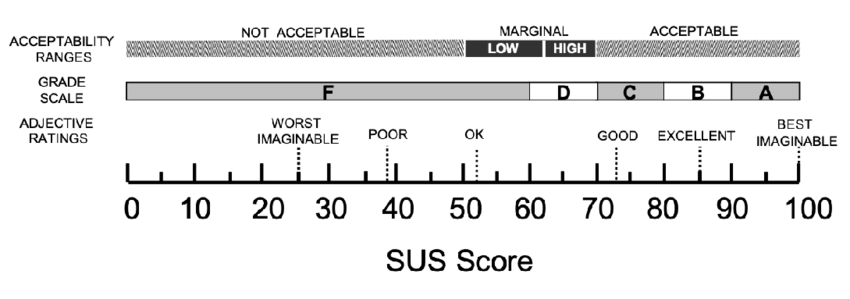
\includegraphics[width=0.8\textwidth]{figures/Grade-rankings-of-SUS-scores-from-An-Empirical-Evaluation-of-the-System-Usability.png}
    \caption{SUS Grade Rankings (adapted from \cite{Bangor2009})}
    \label{fig:sus_scores}
\end{figure}



%%%%%Her må vi vise hvordan kravene er blitt oppfylt med bilder fra dashboardet og linke til spesifikk krav (se incident list lengre ned)
\section{Iterative Development and Functionality Enhancements (RQ2)}
This section addresses the second research question by detailing how the iterative development process, incorporating multiple rounds of feedback and requirement refinement, led to enhanced functionality and better user adaptation.

\subsection{Evolution of Requirements}
Requirement gathering and refinement occurred across four key stages: the initial assignment brief, a stakeholder meeting, as well as user test 1 and 2. Each round added new insight that shaped the system's design and scope. Table~\ref{tab:req_evolution_table} summarises the primary changes introduced during each iteration.

\begin{table}[H]
\centering
\renewcommand{\arraystretch}{1.3}
\resizebox{\textwidth}{!}{
\begin{tabular}{|>{\RaggedRight\arraybackslash}p{4.5cm}|>{\RaggedRight\arraybackslash}p{10.5cm}|}
\hline
\textbf{Development Phase} & \textbf{Main Outcome} \\
\hline
\textbf{Assignment Brief} (\ref{app:req_from_brief}) & Defined the initial scope with five functional (F1–F5) and four non-functional (NF1–NF4) requirements. \\
\hline
\textbf{Stakeholder Meeting} (\ref{app:req_from_stakeholder}) & Clarified user roles and introduced personalised dashboards, resulting in two additional functional requirements (F7–F8). \\
\hline
\textbf{Prototype Testing} (\ref{app:req-prototype}) & Identified UI improvement needs (e.g., colour contrast, filtering/sorting), resulting in new requirements (F9, NF5). \\
\hline
\textbf{MVP User Testing} (\ref{app:req_mvp_user_test}) & Led to the addition of configurable alert thresholds (F10) and a performance constraint (NF6). \\
\hline
\end{tabular}
}
\caption{Key changes in system requirements across development phases}
\label{tab:req_evolution_table}
\end{table}

The full requirement specifications, including those added or modified after each round, are presented in Section~\ref{subsec:req_final}.


\subsection{Functional Enhancements and User Adaptation}
Several new features and refinements were implemented in direct response to feedback across development phases:

\begin{itemize}
    \item \textbf{Filtering and Sorting} (F7): Added after user test 1 to improve content navigation.
    \item \textbf{Configurable Alert Thresholds} (F10): Implemented post-MVP testing to give users control over performance sensitivity.
    \item \textbf{Incident System} (F11): Introduced to highlight and contextualise recurring or critical website issues.
    \item \textbf{User Authentication} (F5): Implemented using JWTs to support personalised dashboards.
    \item \textbf{Improved Navigation and Visual Hierarchies}: Based on feedback that sidebar menus and iconography were unintuitive or cluttered.
\end{itemize}

These enhancements were not only feature additions but also usability refinements based on actual user workflows and preferences. This iterative improvement reflects good human-centred design practice and directly supports RQ2.


% benytt x4development I old for å utfylle seksjonene under
\subsection{System Implementation Outcomes}
\label{subsec:sys_implement_outcomes_results}
The final dashboard system incorporated key technical components that aligned with user needs and design principles.

\subsubsection{System Architecture and Sitemap}
The dashboard followed a modular, multi-page structure, enabling clear navigation between core features such as the main dashboard, website details, and incident tracking. This structure evolved as new functionality was added during iterative development. The final sitemap is shown in Figure~\ref{fig:sitemap_final}.

\begin{figure}[H]
\centering
\includegraphics[width=\textwidth]{figures/Sitemap.png}
\caption{Final sitemap of the application structure and page relationships}
\label{fig:sitemap_final}
\end{figure}

\subsubsection{Monitoring Logic and Alert System}
Monitoring was implemented using \texttt{axios} for HTTP requests and the \texttt{cron} module to trigger status checks at regular intervals. Failures were verified by retrying after 60 seconds. Two  failures resulted in an incident log and an alert, helping users avoid false positives. Users could define thresholds for acceptable response time, and alerts were dispatched only when those constraints were violated. 

\subsubsection{Incident Tracking System}
In response to user test 1 feedback (see Table~\ref{tab:mvp-issues}), The team introduced an updated incident tracking system to allow dashboard users to track and visualise recurring issues to the website they monitor. Incidents were generated based on consecutive monitoring failures and were displayed in both the dashboard and the website details view.

\begin{figure}[H]
\centering
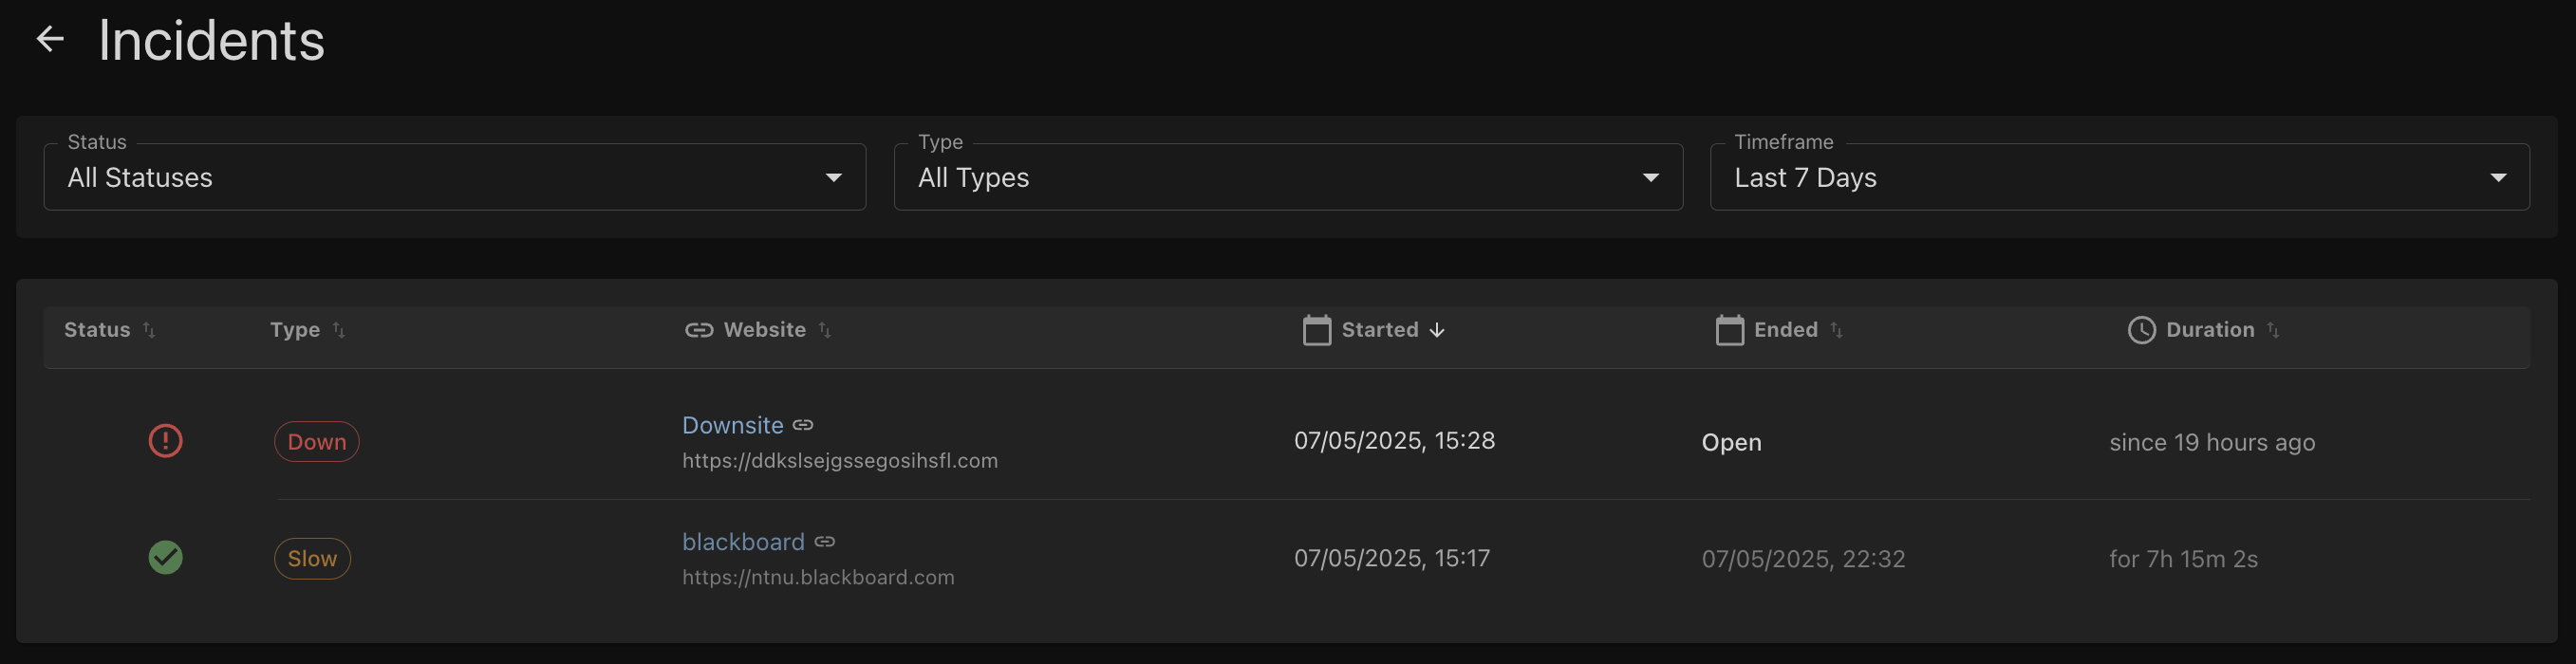
\includegraphics[width=1\textwidth]{figures/IncidentList.png}
\caption{Incident list visualisation in the monitoring dashboard}
\label{fig:incident_list}
\end{figure}

\subsubsection{User Authentication}
User authentication was introduced to support login, registration, and personalised dashboard. This allowed multiple users to manage different sets of websites, improving the system’s scalability and relevance in a real-world team context.

\subsection{Requirement Fulfilment Overview}
\label{subsec:req_final}

To evaluate how well the system met its intended functionality and quality goals, this section reviews the extent to which the defined functional and non-functional requirements were fulfilled. The following tables summarize all requirements as they evolved throughout the project (see \autoref{app:req_from_brief} - \autoref{app:req_mvp_user_test}).


\begin{table}[H]
\centering
\begin{tabular}{|l|p{0.7\linewidth}|l|}
\hline
\textbf{Req ID} & \textbf{Requirement} & \textbf{Priority} \\ \hline
F.1  & Add, edit, and delete monitored websites via the user interface. & High \\ \hline
F.2  & Set custom check intervals per site. & High \\ \hline
F.3  & Display current HTTP status, last response time, and uptime history on each dashboard card. & High \\ \hline
F.4  & Verify that a site is actually up (beyond HTTP 200 status). & High \\ \hline
F.5  & Implement user authentication with personalized dashboards. & Medium \\ \hline
F.6  & Trigger alerts and notifications via e-mail with root cause context. & Medium \\ \hline
F.7  & Provide filtering and sorting of websites. & Medium \\ \hline
F.8  & Add view to easily see change of status per website over time. & High \\ \hline
F.9  & Let users pin websites to the top of the dashboard. & Medium \\ \hline
F.10 & Allow users to configure alert thresholds for performance sensitivity. & Medium \\ \hline
F.11 & Implement an incident tracking system that lists incidents with relevant details. & Medium \\ \hline
F.12 & Allow users to click points on performance graphs to jump directly to related incidents. & Medium \\ \hline
\end{tabular}
\caption{Functional Requirements Defined During the Project}
\label{tab:functional_requirements_full}
\end{table}

% Non-Functional Requirements Table (Consolidated)
\begin{table}[H]
\centering
\begin{tabular}{|l|p{0.7\linewidth}|l|}
\hline
\textbf{Req ID} & \textbf{Requirement} & \textbf{Priority} \\ \hline
NF.1  & Support monitoring of multiple (50+) sites without noticeable delay. & High \\ \hline
NF.2  & Website status changes must be easy to interpret at a glance.  & High \\ \hline
NF.3  & Interface must highlight changes in website status clearly. & High \\ \hline
NF.4  & Code base should be maintainable and well-documented. & Medium \\ \hline
NF.5  & Dashboard card colours must be less overwhelming to the user while still keeping clarity of status. & High \\ \hline
NF.6  & Dashboard data must be updated in near real-time. & High \\ \hline
\end{tabular}
\caption{Non-Functional Requirements Defined During the Project}
\label{tab:nonfunctional_requirements_full}
\end{table}

As shown in Table~\ref{tab:req_fulfilment_matrix}, the system met most core requirements, with several enhancements added after user test 2. A few requirements were partially implemented due to scope constraints or deferred for future development. No high-priority requirements were completely unmet in their final form.

\begin{table}[H]
\centering
\makebox[\textwidth]{
\begin{tabular}{|l|p{0.42\textwidth}|c|c|p{0.30\textwidth}|}
\hline
\textbf{Req ID} & \textbf{Requirement} & \textbf{Priority} & \textbf{Status} & \textbf{Notes} \\ \hline
F.1  & Website CRUD operations & High & ✓ & Fully implemented \\ \hline 
F.2  & Custom check intervals & High & ✓ & -- \\ \hline 
F.3  & Status, response time, uptime display & High & ✓ & -- \\ \hline 
F.4  & Verify site availability beyond HTTP 200 & High & $\sim$ & -- \\ \hline 
F.5  & User authentication & Medium & $\sim$ & Basic login, no roles \\ \hline 
F.6  & Email alerts with root cause context & Medium & ✓ & SMS excluded \\ \hline 
F.7  & Filtering and sorting & Medium & ✓ & Implemented client-side \\ \hline 
F.8  & Historical view (status over time) & High & ✓ & Includes graphs/sparklines \\ \hline 
F.9  & Pin websites to top & Medium & $\sim$ & -- \\ \hline 
F.10 & Configurable alert thresholds & Medium & ✓ & Basic threshold logic added \\ \hline 
F.11 & Incident tracking system & Medium & ✓ & Added after MVP test \\ \hline 
F.12 & Click graph to open related incident & Medium & ✓ & -- \\ \hline 
NF.1 & Support for 50+ sites without delay & High & ✓ & Confirmed in load tests \\ \hline 
NF.2 & Real-time updates and clear status changes & High & ✓ & Includes colour-coding and refresh \\ \hline 
NF.3 & User-friendly interface & High & $\sim$ & Good SUS; mobile issues noted \\ \hline 
NF.4 & Maintainable codebase & Medium & $\sim$ & Some docs/code comments \\ \hline
NF.5 & Visual clarity without overwhelm & High & ✓ & Card layout improved \\ \hline
\end{tabular}
}
\caption{Requirement Fulfilment Matrix}
\label{tab:req_fulfilment_matrix}
\end{table}



\textit{Highlights:} Out of 17 defined requirements, 11 were fully implemented, 4 partially met, and only one entirely unmet. The post-MVP addition of an incident tracking system (F.11) illustrates the iterative responsiveness of the development process.

This overview indicates that the core functionalities and critical non-functional aspects of the monitoring dashboard were successfully delivered. The areas partially met or added post-testing highlight the iterative nature of the development process and provide a basis for discussing design choices, trade-offs, and future improvements in the subsequent chapter.

\section{Summary of Key Findings}
The study demonstrates that applying usability theory and design principles (RQ1) contributed to substantial improvements in dashboard clarity and user experience. A mean \acrshort{sus} score of 85.0 (A grade, 95–97\textsuperscript{th} percentile) reflects a high level of user satisfaction. Qualitative feedback directly informed multiple UI changes, including layout, colour schemes, and visual indicators.

Moreover, iterative development (RQ2) proved effective for aligning the system with real user needs. Requirement refinement, feature additions (e.g., filtering, authentication), and user-centric adjustments were successfully integrated over time.

\section{Addressing the Problem Statement}
The final dashboard embodies the design and functionality goals outlined in the problem statement. Through a structured, user-informed, and theory-grounded development process, the system supports real-time monitoring, intuitive navigation, and meaningful feedback mechanisms. It effectively translates technical performance data into actionable visual insight, aligning with both project objectives and the needs of the end users.

A more detailed discussion of these findings and their implications is presented in the next chapter.
